%% Dokumenteinstellungen %%%%%%%%%%%%%%%%%%%%%%%%%%%%%%%%%%%%
\documentclass[a4paper,oneside,12pt]{scrartcl}

%% Deutsche Anpassungen %%%%%%%%%%%%%%%%%%%%%%%%%%%%%%%%%%%%%
%\usepackage[ngerman]{babel}
\usepackage[T1]{fontenc}
\usepackage[ansinew]{inputenc}
\usepackage{lmodern} %Type1-Schriftart f�r nicht-englische Texte

%% Packages f�r Grafiken & Abbildungen %%%%%%%%%%%%%%%%%%%%%%
\usepackage{graphicx} %%Zum Laden von Grafiken
%\usepackage{subfig} %%Teilabbildungen in einer Abbildung
%\usepackage{tikz} %%Vektorgrafiken aus LaTeX heraus erstellen


%% Packages f�r Formeln %%%%%%%%%%%%%%%%%%%%%%%%%%%%%%%%%%%%%
\usepackage{amsmath}
\usepackage{amsthm}
\usepackage{amsfonts}


%% Andere Packages %%%%%%%%%%%%%%%%%%%%%%%%%%%%%%%%%%%%%%%%%%
%\usepackage{a4wide} %%Kleinere Seitenr�nder = mehr Text pro Zeile.
\usepackage{fancyhdr} %%Fancy Kopf- und Fu�zeilen
%\usepackage{longtable} %%F�r Tabellen, die eine Seite �berschreiten
\usepackage{lastpage}
\usepackage[raggedright]{subfigure}
\usepackage[final]{pdfpages}
\includepdfset{pages=-,noautoscale}

%%%%%%%%%%%%%%%%%%%%%%%%%%%%%%%%%%%%%%%%%%%%%%%%%%%%%%%%%%%%%
%% TODO
%%%%%%%%%%%%%%%%%%%%%%%%%%%%%%%%%%%%%%%%%%%%%%%%%%%%%%%%%%%%%
% 
% 
%%%%%%%%%%%%%%%%%%%%%%%%%%%%%%%%%%%%%%%%%%%%%%%%%%%%%%%%%%%%%



%%%%%%%%%%%%%%%%%%%%%%%%%%%%%%%%%%%%%%%%%%%%%%%%%%%%%%%%%%%%%
%% Optionen / Modifikationen
%%%%%%%%%%%%%%%%%%%%%%%%%%%%%%%%%%%%%%%%%%%%%%%%%%%%%%%%%%%%%
%%%%%%%%%%%%%%%%%%%%%%%%%%%%%%%%%%%%%%%%%%%%%%%%%%%%%%%%%%%%%
%%                                                         %%
%%                     EINSTELLUNGEN                       %%
%%                                                         %%
%%%%%%%%%%%%%%%%%%%%%%%%%%%%%%%%%%%%%%%%%%%%%%%%%%%%%%%%%%%%%

%%%%%%%%%%%%%%%%%%%%%%%%%%%%%%%%%%%%%%%%%%%%%%%%%%%%%%%%%%%%%
%% HYPER REF
%%%%%%%%%%%%%%%%%%%%%%%%%%%%%%%%%%%%%%%%%%%%%%%%%%%%%%%%%%%%%
\usepackage[
hyperindex=true,
colorlinks=true,
linkcolor=black,
citecolor=black,
filecolor=black,
menucolor=black,
urlcolor=cyan,
breaklinks=true,
bookmarks=true,
bookmarksopen=false,
bookmarksnumbered=false,
pdfhighlight=/O,
]{hyperref}

%%%%%%%%%%%%%%%%%%%%%%%%%%%%%%%%%%%%%%%%%%%%%%%%%%%%%%%%%%%%%
%% FANCY HEADERS
%%%%%%%%%%%%%%%%%%%%%%%%%%%%%%%%%%%%%%%%%%%%%%%%%%%%%%%%%%%%%
% --- Kopf- und Fusszeilen - {} = rechts (gerade), [] = links (ungerade)
% letzte seite: \pageref{LastPage}
% doppelseitig:
%\lhead{Elektronik: \textbf{Oszilatorschaltungen}}	\chead{}		\rhead{Cyril Stoller und Hannes Stauffer}
%\lfoot{\today}	\cfoot{}		\rfoot{Seite \thepage\ von \pageref{LastPage}}

% einseitig:
%\lhead{\rightmark}			\chead{}					\rhead{}
%\lfoot{\leftmark}			\cfoot{}					\rfoot{Seite \thepage\ von \pageref{\LastPage}}

%\setlength{\headrulewidth}{0.4pt}
%\setlength{\footrulewidth}{0.4pt}


%%%%%%%%%%%%%%%%%%%%%%%%%%%%%%%%%%%%%%%%%%%%%%%%%%%%%%%%%%%%%
%% DOKUMENT
%%%%%%%%%%%%%%%%%%%%%%%%%%%%%%%%%%%%%%%%%%%%%%%%%%%%%%%%%%%%%
\begin{document}

\title{Praktikum 4.2: Aktives Filter}
\date{\today}
\author{Cyril Stoller, Marcel B�rtschi}
\maketitle

%% Inhaltsverzeichnis %%%%%%%%%%%%%%%%%%%%%%%%%%%%%%%%%%%%%%%
\tableofcontents %Inhaltsverzeichnis

%\pagestyle{fancy} %%Ab hier die Kopf-/Fusszeilen: headings / fancy / ...

\vspace{2cm}

\begin{abstract}
	
\begin{center}	
\textbf{Abstract}
\vspace{0.3cm}

	Dieser Bericht ist erg�nzend zum Laborjournal und enth�lt vertiefte Diskussion der gemessenen Resultate, sowie die detailierten Berechnungen.
\end{center}
	
\end{abstract}

\vspace{2cm}


%%%%%%%%%%%%%%%%%%%%%%%%%%%%%%%%%%%%%%%%%%%%%%%%%%%%%%%%%%%%%
%%                                                         %%
%%         Kapitel / Hauptteil des Dokumentes              %%
%%                                                         %%
%%%%%%%%%%%%%%%%%%%%%%%%%%%%%%%%%%%%%%%%%%%%%%%%%%%%%%%%%%%%%



\section{Ziel}

Dieser Bericht beinhaltet genaue Angaben zur Durchf�hrung und eine Diskussion des Versuches Aktive Filter im Modul BTE5032.02. Es soll ein aktives Filter dimensioniert, aufgebaut und ausgemessen werden. Die Resultate sollen anschliessend mit Resultaten aus einer Simulation verglichen und diskutiert werden.

\section{Einleitung}

\subsection{Motivation}
Die im letzten Semester erlernte Filtertheorie soll mit diesem Praktikum in der Praxis nachvollzogen und zu vertieft werden. Ausserdem soll w�hrend dem Praktikum ein Laborjournal gef�hrt werden. Dies soll soweit ge�bt werden, dass es im Arbeitsalltag als Elektroingenieur zur Gewohnheit wird.

\subsection{Aufgabenstellung}
Die Aufgabenstellung ist unter \url{http://moodle.bfh.ch/course/view.php?id=3380} oder im Anhang zu finden.

\section{Durchf�hrung}

\subsection{Theorie}
Ein aktives Filter besteht aus einem OpAmp mit einer Beschaltung aus Kondensatoren und Widerst�nden. Es hat verglichen zum passiven Filter (welches ausschliesslich aus diskreten Elementen wie Widerst�nden, Kondensatoren und Spulen) die Vorteile, dass es einfacher h�here Ordnungen erzielen kann und eine Verst�rkung enth�lt.

\begin{figure}[ht]
	\centering
		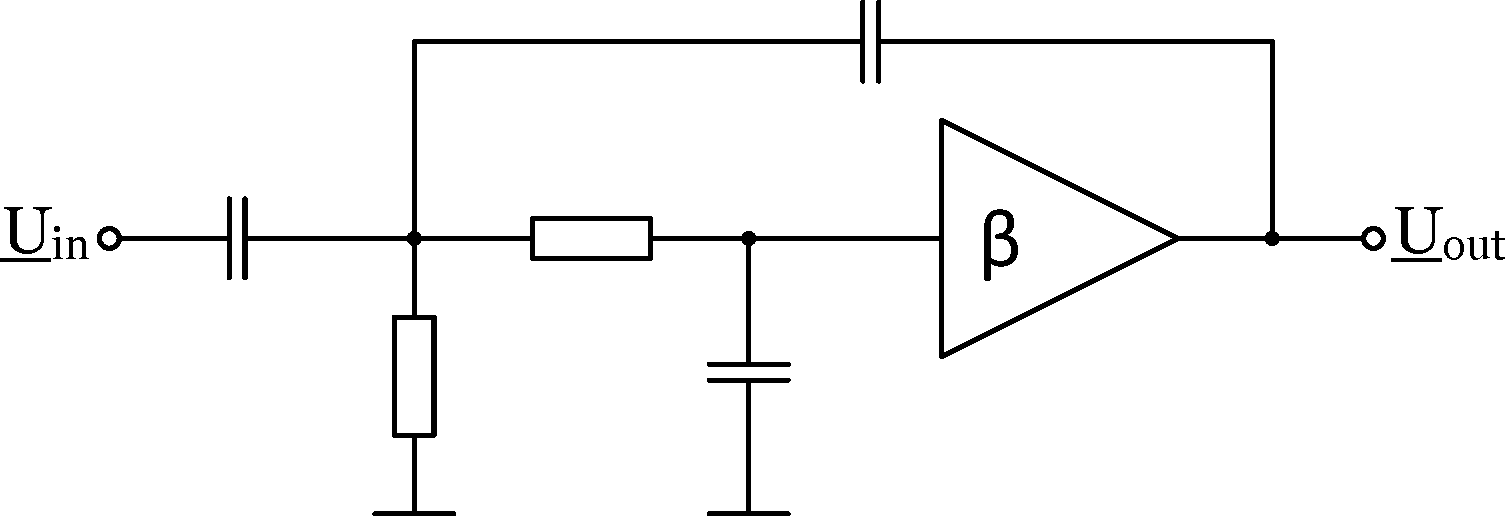
\includegraphics[width=0.60\textwidth]{images/Konzeptschema.pdf}
	\caption[Konzeptschema des Bandpasses zweiter Ordnung]{Konzeptschema des Bandpasses zweiter Ordnung\cite{konzeptschema}}
	\label{konzeptschema}
\end{figure}

Hier verwenden wir ein Bandpassfilter zweiter Ordnung (siehe Abb. \ref{konzeptschema}). Der Verst�rkerblock mit der Bezeichnung $\beta$ ist im Prinzip eine nicht-invertierende OpAmp-Verst�rkerschaltung mit einer Offset-Kompensation.

\subsection{Dimensionierung}
Bei der Dimensionierung sind wir genau nach der Aufgabenstellung gegangen. Zuerst haben wir das $\beta$ berechnet.

Um die Werte genau zu erreichen, haben wir bei den Widerst�nden R1 und R3 zus�tzlich ein Potentiometer in Serie geschaltet. Somit bleibt einen gewisser Spielraum um die Schaltung sauber abzustimmen.

\begin{figure}[ht]
	\centering
		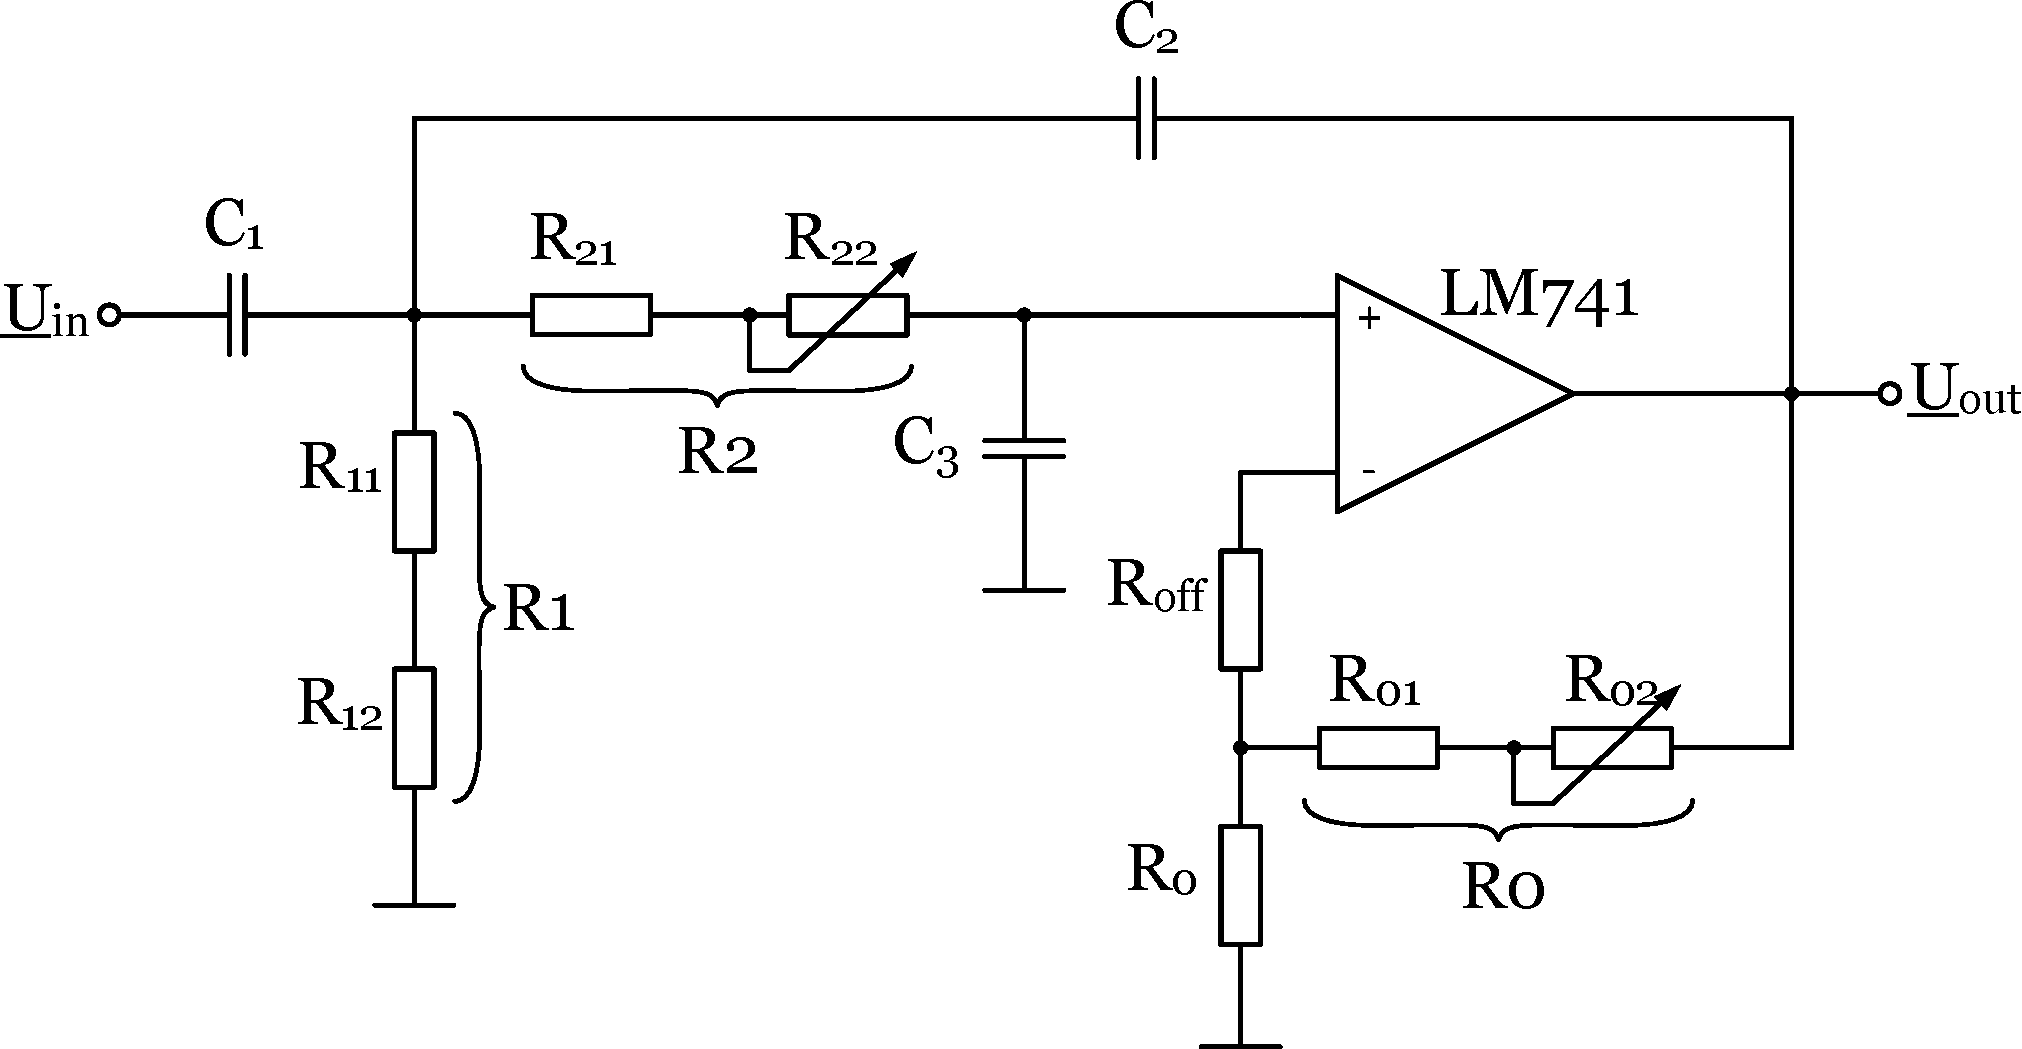
\includegraphics[width=0.80\textwidth]{images/Schema.pdf}
	\caption{Schema f�r den Aufbau}
	\label{schema}
\end{figure}

\subsection{Simulation}
Die Simulation wurde in LT Spice durchgef�hrt. Da in der Aufgabenstellung der OpAmp LM741 vorgegeben ist, mussten wir diesen zuerst noch im Spice hinzuf�gen. 
Danach die Simulation gem�ss dem Schema aufbauen und die Werte entsprechend der Dimensionierung w�hlen. Die Widerst�nde haben wir in der Simulation genau auf den berechneten Wert eingestellt. Bei der realen Schaltung haben wir einen N�herungswert genommen und mit einem Potentiometer in Serie zum Widerstand den Wert genau abgeglichen.


\subsection{Aufbau}
Der Aufbau auf der Steckplatte hat uns am meisten Schwierigkeiten bereitet. Gleich zwei mal hatten wir einen Fehler im Aufbau. 
\begin{figure}[ht]
	\centering
		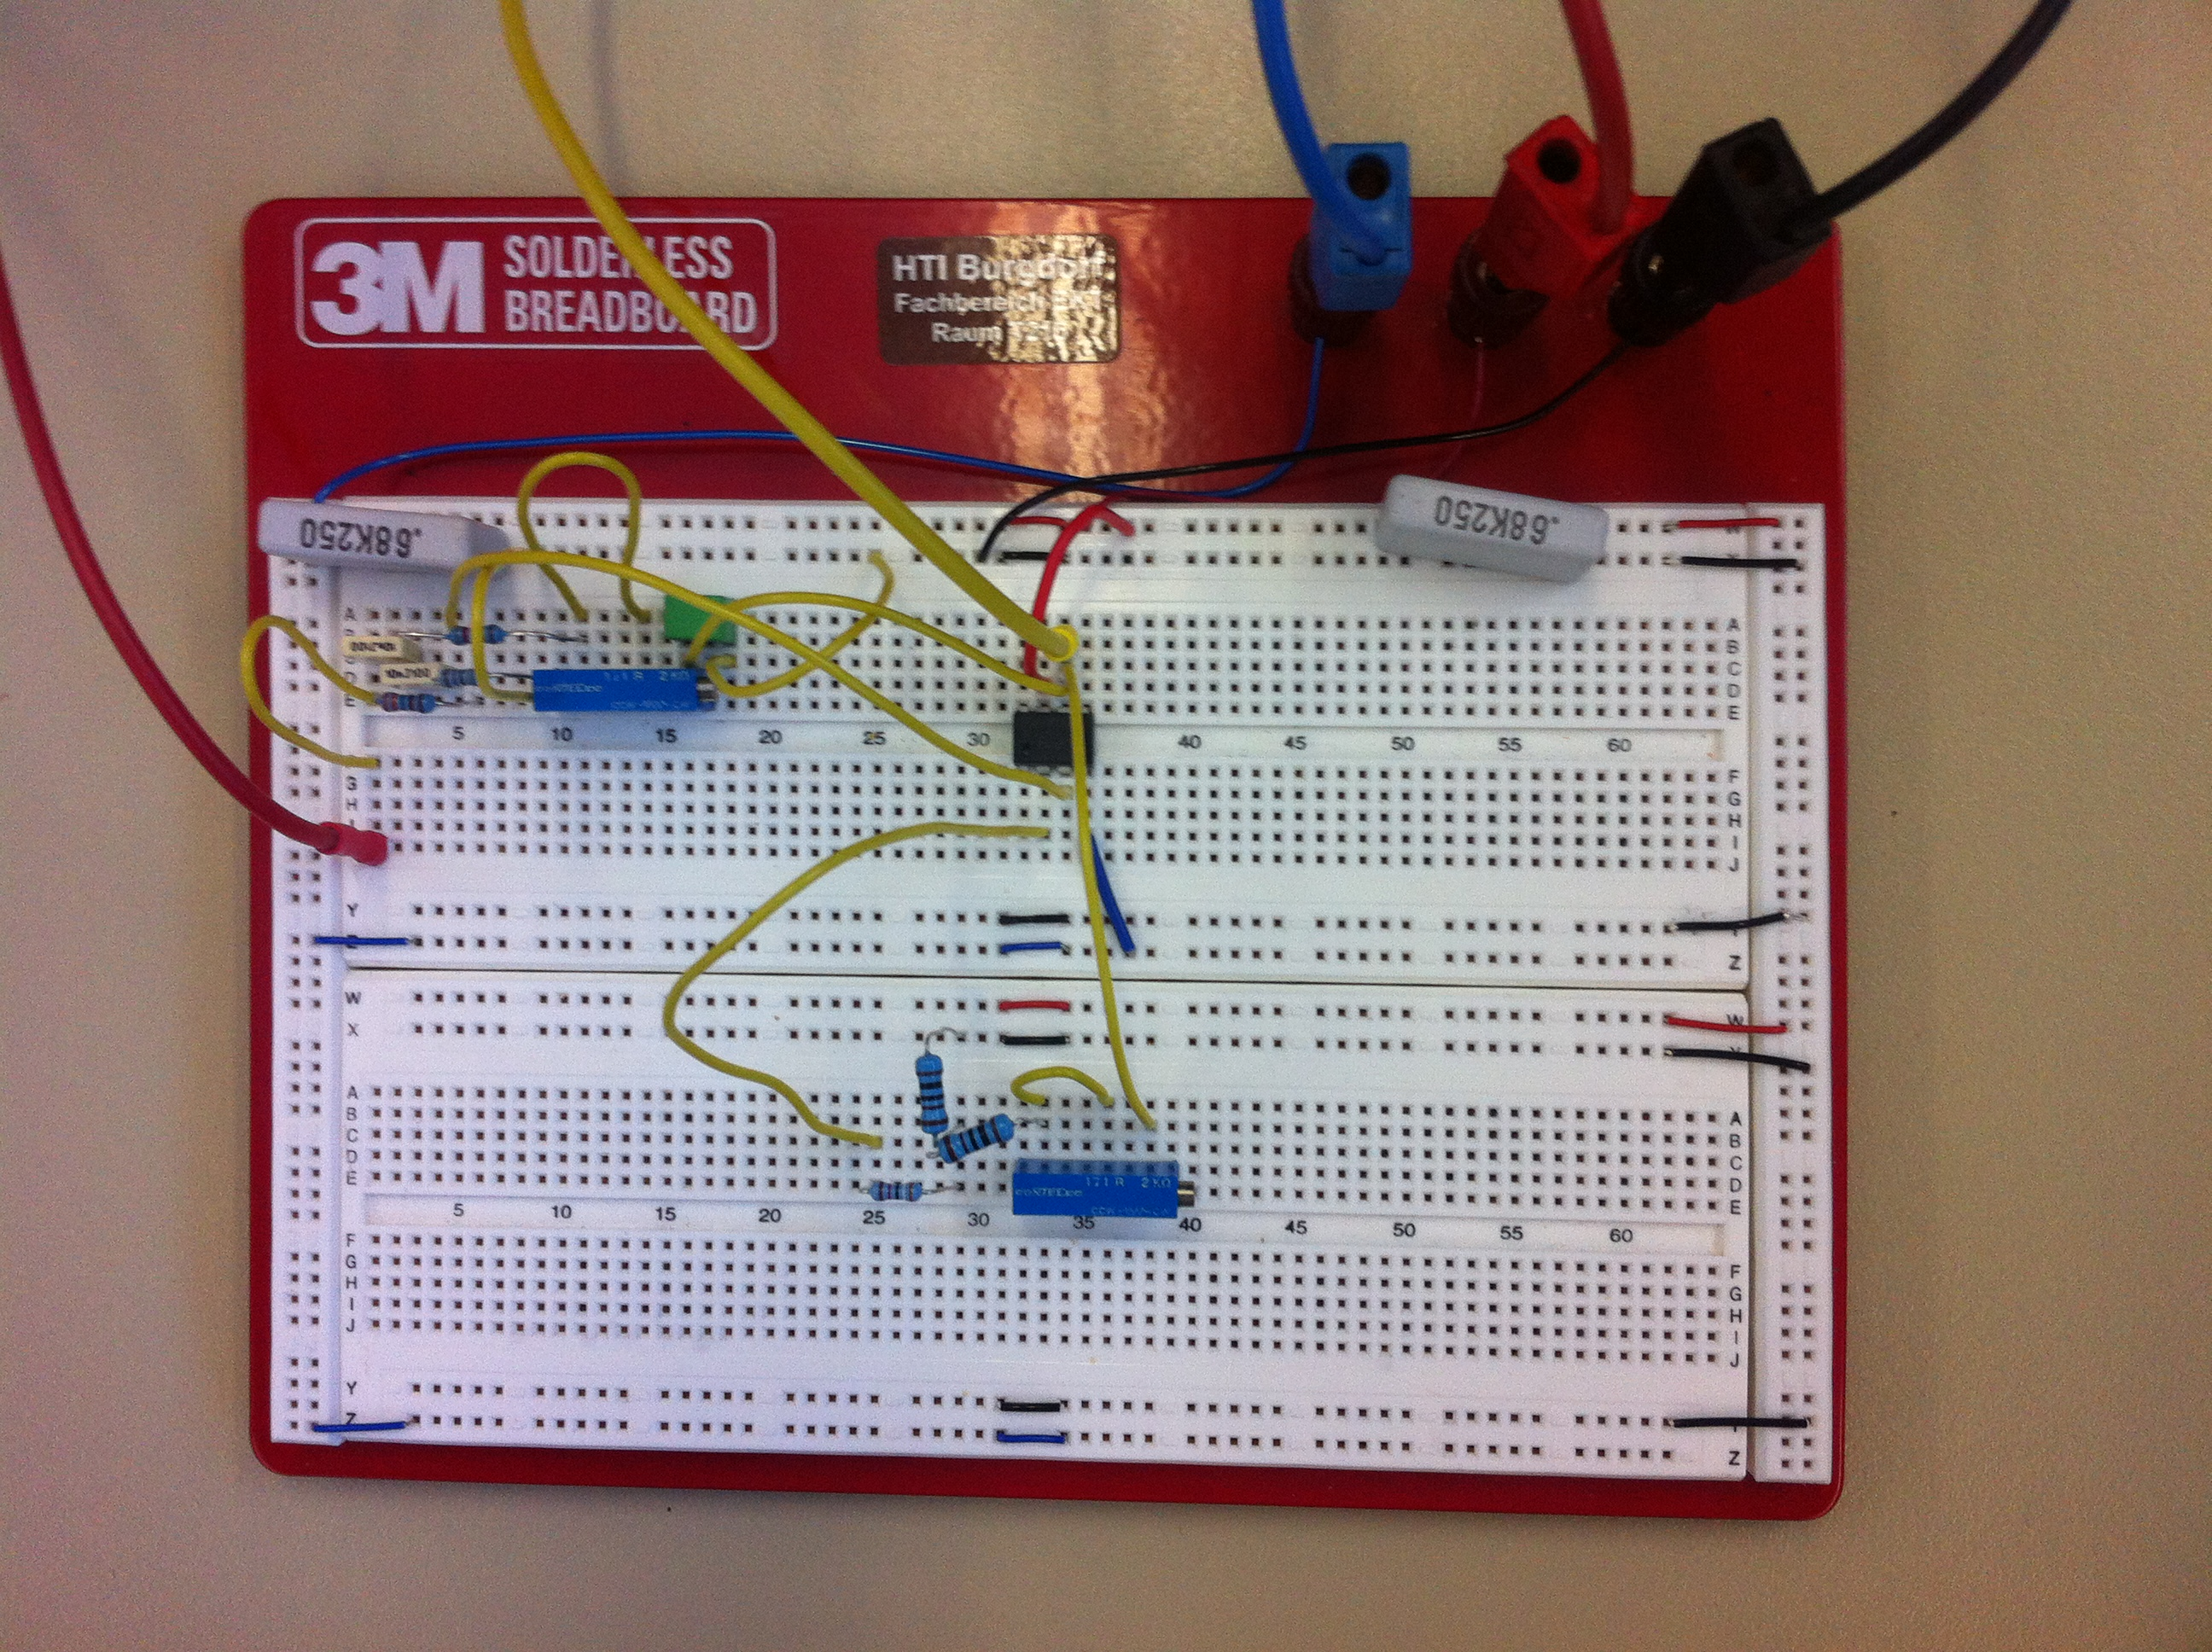
\includegraphics[width=0.80\textwidth]{images/Foto 2.jpg}
	\caption[Aufbau auf der Steckplatte]{Aufbau auf der Steckplatte\cite{Aufbau}}
	\label{Aufbau}
\end{figure}
\subsection{Abstimmung}

\subsubsection{Mittenfrequenz}
Wir speisen am Eingang die Mittenfrequenz ein und messen am Ausgang die Phase. Da die Amplitude in der N�he der Mittenfrequenz recht flach ist, kann man damit schlecht abstimmen. Laut dem erwarteten Phasengang eines Bandpasses wird sich dort die Phase aber schnell �ndern und bei perfekter Abstimmung bei 45� sein.

\subsection{Messung}
Messmittelliste ist im Anhang zu finden.

\subsection{Fehlerabsch�tzung}

\subsection{Diskussion}


\section{Schlussfolgerung}
Als Fazit k�nnen wir sagen, dass wir mit Hilfe der Anleitung die Dimensionierung gut durchf�hren konnten. Leider haben wir beim Aufbau zu viel Zeit verloren, die uns danach gefehlt hat, um die Auswertung noch detaillierter zu gestalten. So hatten wir zum Beispiel keine Zeit mehr die G�te anhand der Bandbreite und der Mittenfrequenz nachzukontrollieren. 



\section*{Quellenverzeichnis}

\renewcommand\refname{Quellenverzeichnis}
\bibliographystyle{amsplain}
\bibliography{Bildquellen}

\listoffigures

% Der Anhang kommt auf eine neue Zeile
\newpage
% Offizielle "A Anhang" Aufz�hlungsvariante
\appendix
% Nur im Inhaltsverzeichnis hinzuf�gen (mit richtiger Seite, da vorher "\newpage"), aber kein Text
\addcontentsline{toc}{section}{Anhang}

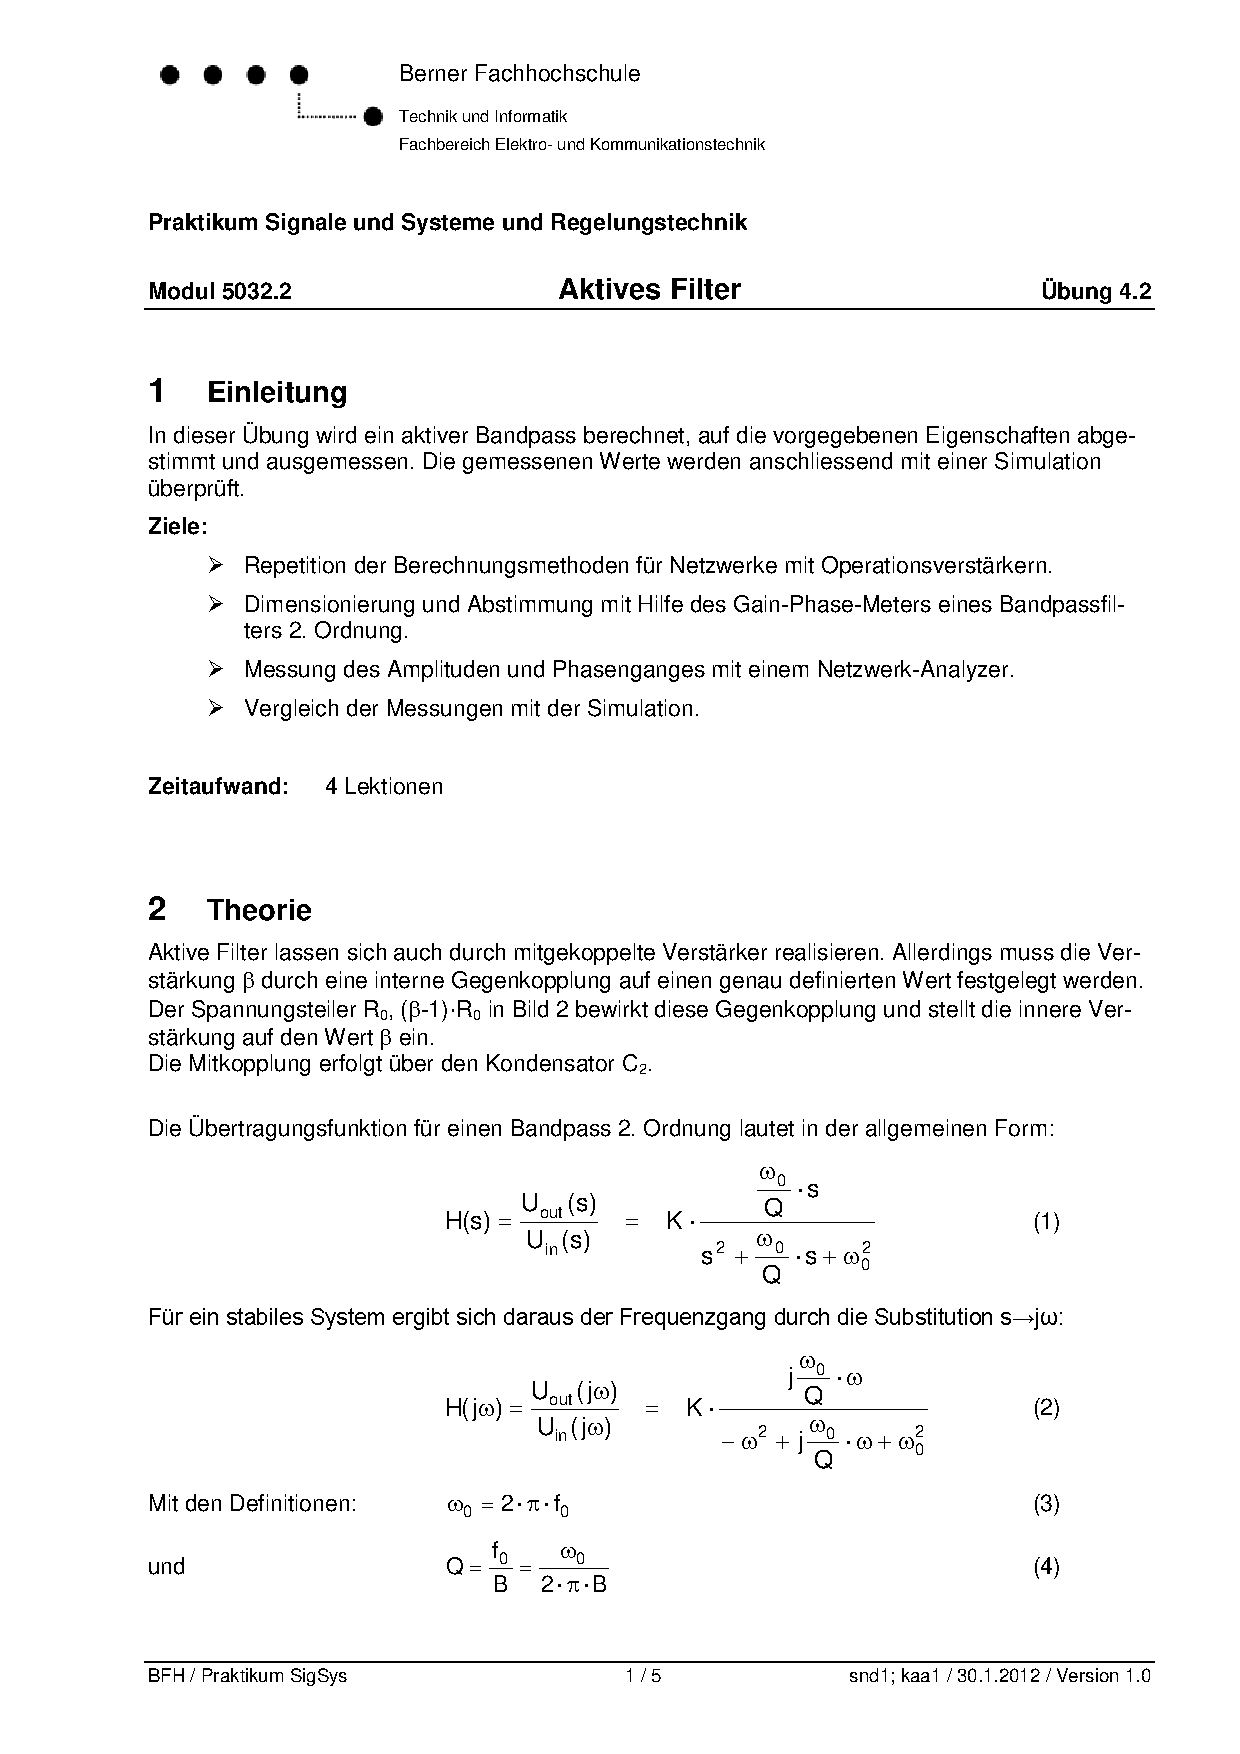
\includepdf{Praktikumsunterlagen.pdf}

\end{document}
